\documentclass[a4paper, 12pt]{article}
\usepackage[utf8x]{inputenc}
\usepackage[english, russian]{babel}
\usepackage[left=25mm, top=25mm, right=25mm, bottom=25mm]{geometry}
\usepackage{cmap}
\usepackage{indentfirst}
\usepackage{tikz}
\usepackage{float}
\usepackage{amsmath, amsfonts, amssymb}
\usepackage{graphicx}
\usepackage{hyperref}
\usepackage{listings}
\usepackage{caption}
\usepackage{subcaption}
\usepackage{xcolor}
\usepackage{etoolbox}
\usepackage{titlesec}
\pagestyle{plain}
\patchcmd{\tableofcontents}{\contentsname}{\centering\contentsname}{}{}
\titleformat{\section}[block]{\normalfont\large\bfseries\centering}{}{0pt}{}
\titleformat{\subsection}[block]{\normalfont\normalsize\bfseries\centering}{}{0pt}{}
\allowdisplaybreaks
\graphicspath{{src/images/}}
\usetikzlibrary{patterns}
\definecolor{LightGray}{gray}{0.95}
\definecolor{LightGray2}{gray}{0.7}
\lstdefinestyle{code}{
    language=MATLAB, % replace language here
    basicstyle=\footnotesize\ttfamily,
    % numbers=left,
    % numberstyle=\scriptsize\color{gray},
    % stepnumber=1,
    % numbersep=5pt,
    backgroundcolor=\color{LightGray},
    showspaces=false,
    showstringspaces=false,
    showtabs=false,
    tabsize=4,
    captionpos=b,
    breaklines=true,
    breakatwhitespace=false,
    frame=single,
    rulecolor=\color{LightGray2},
    linewidth=\linewidth,
    keywordstyle=\color{blue}\bfseries,
    commentstyle=\color{green!40!black},
    stringstyle=\color{purple},
    escapeinside={\%*}{*)},
    inputencoding=utf8x,
    xleftmargin=0pt,
    framexleftmargin=0pt,
    framexrightmargin=0pt
}
\lstset{style=code}
\hypersetup{
    colorlinks=true,
    linkcolor=blue,
    filecolor=magenta,
    urlcolor=cyan,
    pdftitle={contents setup},
    pdfpagemode=FullScreen,
}


\begin{document}
    \begin{titlepage}

        \begin{center}
        Федеральное государственное автономное образовательное учреждение высшего образования
        «Национальный Исследовательский Университет ИТМО»
        \vfill
        
        
\includegraphics[width=0.3\textwidth]{itmo.png} % requires /src/images/itmo.png

        {\large\bf ЛАБОРАТОРНАЯ РАБОТА №3}\\
        {\large\bf ПРЕДМЕТ «ТЕОРИЯ АВТОМАТИЧЕСКОГО УПРАВЛЕНИЯ»}\\
        {\large\bf ТЕМА «РЕГУЛЯТОРЫ С ЗАДАННОЙ СТЕПЕНЬЮ УСТОЙЧИВОСТИ»}\\
        Вариант №2
        \vfill

        \begin{flushright}
            \begin{minipage}{.45\textwidth}
            {
                \hbox{Преподаватель:}
                \hbox{Пашенко А. В.}
                \hbox{}
                \hbox{Выполнил:}
                \hbox{Румянцев А. А.}
                \hbox{}
                \hbox{Факультет: СУиР}
                \hbox{Группа: R3341}
                \hbox{Поток: ТАУ R22 бак 1.1.1}
            }
            \end{minipage}
        \end{flushright}
        \vfill
  
        Санкт-Петербург\\
        2025
        \end{center}
    \end{titlepage}
    
    \tableofcontents

    \newpage
    \section{Задание 1. Синтез регулятора с заданной степенью устойчивости}
    Рассмотрим систему
    $$
    \dot{x}=Ax+Bu,\ A=\begin{bmatrix}
        5 &2 &7\\
        2 &1 &2\\
        -2 &-3 &-4
    \end{bmatrix},\ B=\begin{bmatrix}
        3\\1\\-1
    \end{bmatrix};
    $$


    \subsection{Управляемость и стабилизируемость}
    Найдем собственные числа матрицы $A$ и определим управляемость каждого из них. Программа для
    вычислений в \texttt{MATLAB} представлена на листинге \ref{task1code} в приложении А
    $$
    \sigma\left( A \right)=\left\{-2,2\pm i\right\}
    $$
    Число $\lambda_1=-2$ асимптотически устойчивое, может быть неуправляемым. Комплексная пара $\lambda_{2,3}$
    имеет положительную действительную часть -- эти собственные числа неустойчивые, нужна управляемость.
    Разложим $A$ в вещественную жорданову форму, найдем вектор $B$ в базисе собственных векторов матрицы $A$
    $$
    A=P_{re}J_{re}P_{re}^{-1}=\begin{bmatrix}
    -1    &0.5   &-1.5\\
    0         &0   &-1\\
    1         &0    &1
    \end{bmatrix}\begin{bmatrix}
    -2     &0     &0\\
     0     &2     &1\\
     0    &-1     &2
    \end{bmatrix}\begin{bmatrix}
    0     &1     &1\\
     2    &-1     &2\\
     0    &-1     &0
    \end{bmatrix},
    $$
    $$
    B_{Jre}=P_{re}^{-1}B=\begin{bmatrix}
        0     &1     &1\\
         2    &-1     &2\\
         0    &-1     &0
        \end{bmatrix}\begin{bmatrix}
            3\\
            1\\
            -1
        \end{bmatrix}=\begin{bmatrix}
        0\\
     3\\
    -1
    \end{bmatrix};
    $$
    Итого имеем
    $$
    J_{re}=\begin{bmatrix}
        -2     &0     &0\\
         0     &2     &1\\
         0    &-1     &2
        \end{bmatrix},\ B_{Jre}=\begin{bmatrix}
            0\\
         3\\
        -1
        \end{bmatrix};
    $$
    Все жордановы клетки относятся к различным собственным числам. Только число $\lambda_1=-2$ неуправляемое,
    так как первый элемент $B_{Jre}$ равен нулю. Остальные собственные числа управляемые. Таким образом,
    система не полностью управляема, стабилизируема.


    \subsection{Степень устойчивости}
    Любой степени устойчивости при помощи регулятора $u=Kx$ добиться не получится, так как система не полностью управляема.
    Степень устойчивости системы $\alpha$ -- самое близкое
    к правой комплексной полуплоскости собственное число матрицы $A$,
    находящееся в левой комплексной полуплоскости. Проверка на близость
    осуществляется через действительную часть собственного числа. Имеем
    $$
    \text{Re}\left\{ \lambda_1=-2 \right\}=-2,
    $$
    $$\text{Re}\left\{ \lambda_{2,3}=2\pm i \right\}=2;
    $$
    Таким образом, степень устойчивости системы $\alpha=2$. Это максимум. Устойчивость в данном случае
    подразумевается экспоненциальная.


    \subsection{Схема моделирования системы, замкнутой регулятором}
    Построим схему моделирования системы $\dot{x}=Ax+Bu$, замкнутой регулятором $u=Kx$, используя \texttt{SIMULINK}
    \begin{figure}[H]
        \centering
        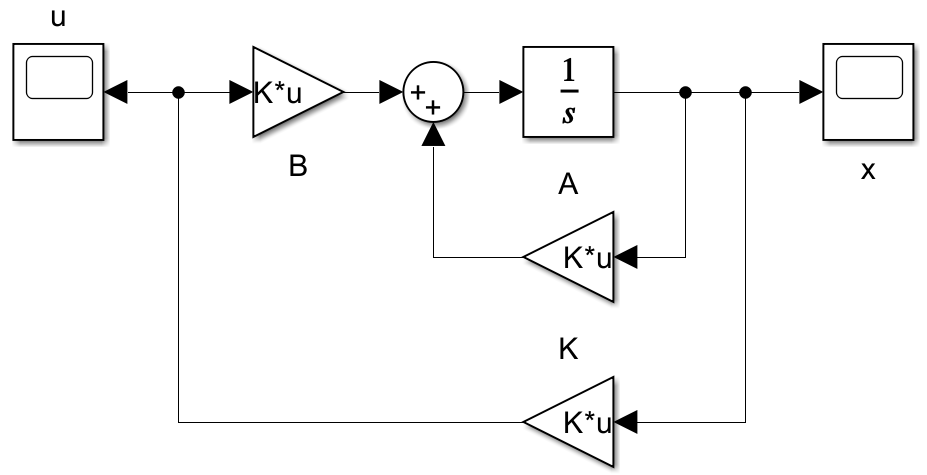
\includegraphics[scale=0.5]{scheme_task1.png}
        \captionsetup{skip=0pt}
        \caption{Схема моделирования системы, замкнутой регулятором}
        \label{fig:scheme_task1}
    \end{figure}


    \subsection{Значения желаемой степени устойчивости}
    Возьмем достаточно отличающиеся достижимые степени устойчивости в диапазоне $0<\alpha\leq2$
    \begin{align*}
        &\alpha_{1}=2,\\
        &\alpha_2=0.1;
    \end{align*}


    \subsection{Синтез регулятора через матричное неравенство типа Ляпунова}
    Для каждого из выбранных значений $\alpha$ синтезируем регулятор, обеспечивающий
    заданную степень устойчивости, при помощи матричного неравенства типа Ляпунова
    $$
    PA^T+AP+2\alpha P+Y^TB^T+BY\preceq0,\ K=YP^{-1};
    $$


    Найдем для $\alpha_{1,2}$ соответствующие матрицы регулятора $K_{1\,\alpha_i}$ \textbf{без ограничений на управление}.
    Пользуемся пакетом \texttt{cvx} для \texttt{MATLAB}. Получаем
    $$
    K_{1\,\alpha_1}=\begin{bmatrix}
        2.5267  &-18.8652    &1.7294
    \end{bmatrix},
    $$
    $$
    K_{1\,\alpha_2}=\begin{bmatrix}
        -2.0955   &-5.8106   &-2.6863
    \end{bmatrix};
    $$


    Найдем для $\alpha_{1,2}$ соответствующие матрицы регулятора $K_{2\,\alpha_i}$ \textbf{совместно с решением задачи минимизации управления}.
    Нам нужно найти минимальное $\mu$, для которого при начальных условиях $x(0)=x_0$
    выполняется $||u(t)||\leq\mu$. Для этого нужно решить задачу выпуклой минимизации:
    \begin{align*}
    &\text{минимизировать }\gamma=\mu^2\\
    &\text{при ограничениях } P\succ0,\ PA^T+AP+2\alpha P+Y^TB^T+BY\prec0,\\
    &\begin{bmatrix}
        P &x_0\\
        x_0^T &1
    \end{bmatrix}\succ0,\ \begin{bmatrix}
        P &Y^T\\
        Y &\gamma I
    \end{bmatrix};
    \end{align*}
    Зададим начальные условия $$x(0)=\begin{bmatrix}
        1 \\1 \\1
    \end{bmatrix}$$
    Реализация представлена в \texttt{MATLAB}, для решения используется \texttt{cvx}. Получаем
    $$
    K_{2\,\alpha_1}=\begin{bmatrix}
        1.6000  &-11.2000    &1.6000
    \end{bmatrix},\ \mu_1=8.0090,
    $$
    $$
    K_{2\,\alpha_2}=\begin{bmatrix}
        -0.7565   &-2.6884   &-0.7552
    \end{bmatrix},\ \mu_2=4.2015;
    $$


    Определим собственные числа матриц замкнутых систем $\left( A+BK_{j\,\alpha_i} \right)$
    и сравним с желаемой степенью устойчивости
    \begin{align*}
    &\sigma\left( A+BK_{1\,\alpha_1} \right)=\left\{ -2, -4.5072\pm3.2145i \right\},\\
    &\sigma\left( A+BK_{1\,\alpha_2} \right)=\left\{ -2,-4.5455,-0.8653 \right\},\\
    &\sigma\left( A+BK_{2\,\alpha_1} \right)=\left\{ -2, -2.0000\pm4.1231i \right\},\\
    &\sigma\left( A+BK_{2\,\alpha_2} \right)=\left\{ -2,-0.1013\pm2.3259i \right\};
    \end{align*}
    Для $\alpha_1=2$ собственные числа при регуляторе $K_{2\,\alpha_1}$ получились более точными,
    чем при регуляторе $K_{1\,\alpha_1}$. То есть управление будет именно таким, каким мы его хотели $\left( \text{Re}\left\{ \lambda_i \right\}=-\alpha_1 \right)$.
    На графике увидим плавное поведение системы, стабилизирующееся к нулю. Для $\alpha_2=0.1$ ситуация аналогичная
    -- при $K_{2\,\alpha_2}$ действительная часть комплексной пары почти достигла желаемого ограничения на степень устойчивости.
    При $K_{2\,\alpha_2}$ результат более хаотичный. Также в каждом спектре наблюдаем неуправляемое число $-2$, что подтверждает
    корректность расчетов.


    \subsection{Компьютерное моделирование}
    Выполним компьютерное моделирование для всех замкнутых систем, используя схему \texttt{SIMULINK},
    представленную на рис. \ref{fig:scheme_task1}. Построим графики $u(t),x(t)$ при начальных условиях
    $$x(0)=\begin{bmatrix}
        1 \\1 \\1
    \end{bmatrix}$$ и сопоставим результаты.

    
    Графики представлены далее на рис. \ref{fig:1task_K1a1_u}--\ref{fig:1task_K2a2_x}
    \newpage
    \vspace*{0.01mm}
    \begin{figure}[H]
        \centering
        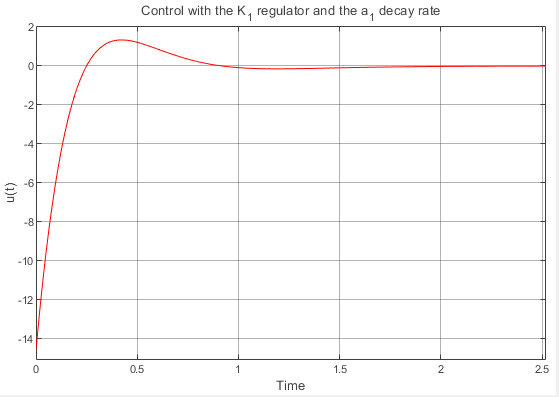
\includegraphics{1task_K1a1_u.png}
        \captionsetup{skip=0pt}
        \caption{График $u(t)$ для $\alpha_1=2$ при $K_{1\,\alpha_1}$}
        \label{fig:1task_K1a1_u}
    \end{figure}
    \begin{figure}[H]
        \centering
        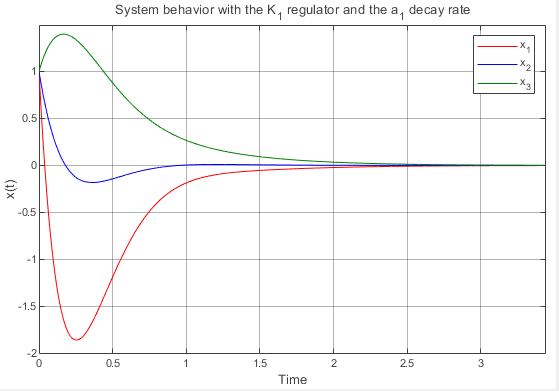
\includegraphics{1task_K1a1_x.png}
        \captionsetup{skip=0pt}
        \caption{График $x(t)$ для $\alpha_1=2$ при $K_{1\,\alpha_1}$}
        \label{fig:1task_K1a1_x}
    \end{figure}
    \newpage
    \vspace*{0.01mm}
    \begin{figure}[H]
        \centering
        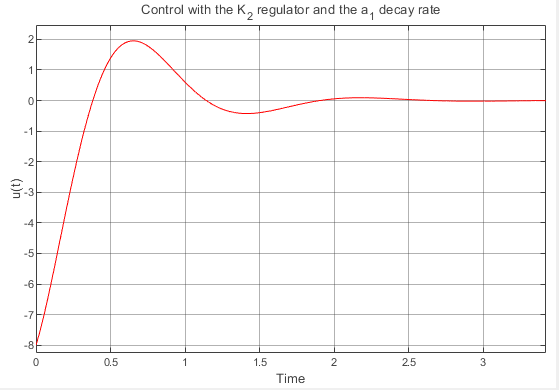
\includegraphics{1task_K2a1_u.png}
        \captionsetup{skip=0pt}
        \caption{График $u(t)$ для $\alpha_1=2$ при $K_{2\,\alpha_1},\ \mu_1=8.0090$}
        \label{fig:1task_K2a1_u}
    \end{figure}
    \begin{figure}[H]
        \centering
        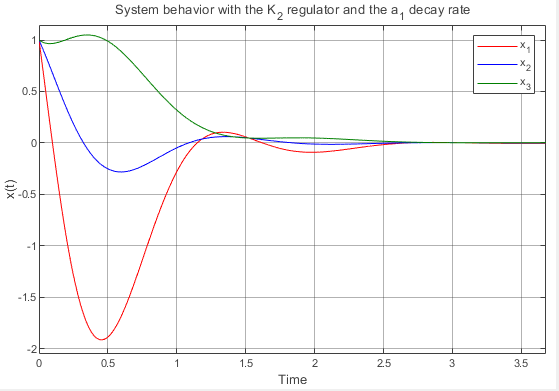
\includegraphics{1task_K2a1_x.png}
        \captionsetup{skip=0pt}
        \caption{График $x(t)$ для $\alpha_1=2$ при $K_{2\,\alpha_1},\ \mu_1=8.0090$}
        \label{fig:1task_K2a1_x}
    \end{figure}
    \newpage
    \vspace*{0.01mm}
    \begin{figure}[H]
        \centering
        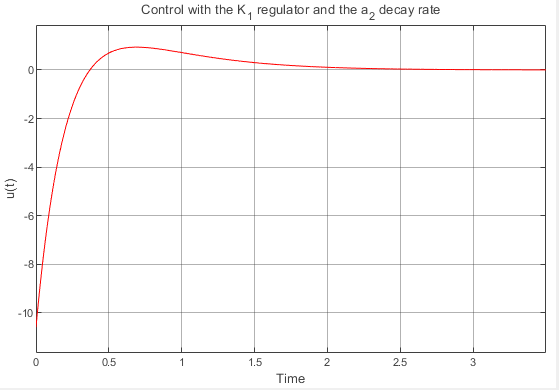
\includegraphics{1task_K1a2_u.png}
        \captionsetup{skip=0pt}
        \caption{График $u(t)$ для $\alpha_2=0.1$ при $K_{1\,\alpha_2}$}
        \label{fig:1task_K1a2_u}
    \end{figure}
    \begin{figure}[H]
        \centering
        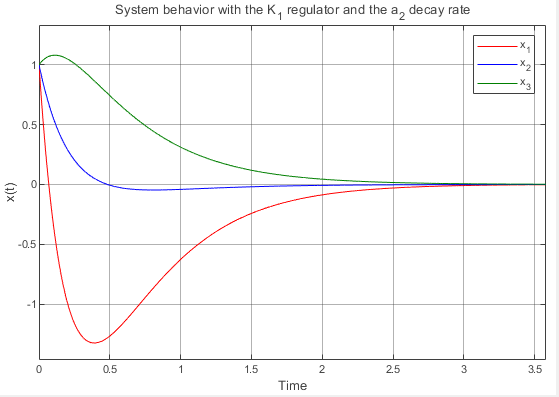
\includegraphics{1task_K1a2_x.png}
        \captionsetup{skip=0pt}
        \caption{График $x(t)$ для $\alpha_2=0.1$ при $K_{1\,\alpha_2}$}
        \label{fig:1task_K1a2_x}
    \end{figure}
    \newpage
    \vspace*{0.01mm}
    \begin{figure}[H]
        \centering
        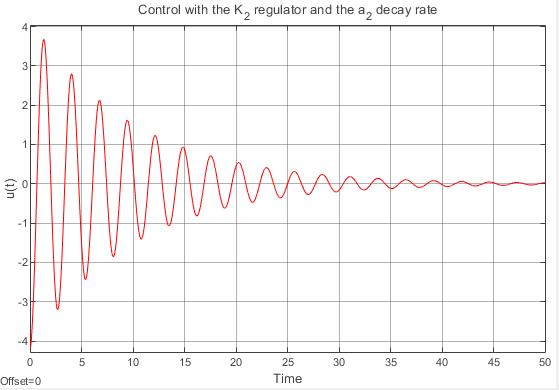
\includegraphics{1task_K2a2_u.png}
        \captionsetup{skip=0pt}
        \caption{График $u(t)$ для $\alpha_2=0.1$ при $K_{2\,\alpha_2},\ \mu_2=4.2015$}
        \label{fig:1task_K2a2_u}
    \end{figure}
    \begin{figure}[H]
        \centering
        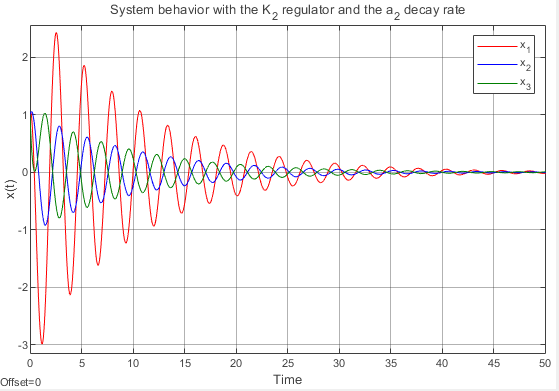
\includegraphics{1task_K2a2_x.png}
        \captionsetup{skip=0pt}
        \caption{График $x(t)$ для $\alpha_2=0.1$ при $K_{2\,\alpha_2},\ \mu_2=4.2015$}
        \label{fig:1task_K2a2_x}
    \end{figure}


    \subsection{Сопоставление результатов}
    На рис. \ref{fig:1task_K2a1_u}, \ref{fig:1task_K2a2_u} видим, что систему удается стабилизировать при помощи минимального управления,
    однако на это уходит больше времени, что наблюдается при сравнении поведения систем на рис. \ref{fig:1task_K2a2_x}, \ref{fig:1task_K1a2_x}.
    В случае с рис. \ref{fig:1task_K2a1_x}, \ref{fig:1task_K1a1_x} это менее заметно. В общем результаты без ограничения на управление более гладкие
    и спокойные, но требуют больше управления.


    \subsection{Синтез регулятора через матричное уравнение типа Риккати}
    Для каждого $\alpha$ синтезируем регулятор при помощи матричного уравнения типа Риккати при $\nu=2\text{ и }R=1$
    $$
    A^TP+PA+Q-\nu PBR^{-1}B^TP+2\alpha P=0,\,K=-R^{-1}B^TP;
    $$
    Пользуемся \texttt{MATLAB}. Найдем матрицы регулятора $K_{3\,\alpha_i}$ при $Q=I$
    $$
    K_{3\,\alpha_1}=\begin{bmatrix}
        2.1164  &-13.4942    &1.6777
    \end{bmatrix},
    $$
    $$
    K_{3\,\alpha_2}=\begin{bmatrix}
        -0.8455   &-3.3716   &-0.5697
    \end{bmatrix};
    $$
    Найдем матрицы регулятора $K_{4\,\alpha_i}$ при $Q=0$
    $$
    K_{4\,\alpha_1}=\begin{bmatrix}
        1.6000  &-11.2000    &1.6000
    \end{bmatrix},
    $$
    $$
    K_{4\,\alpha_2}=\begin{bmatrix}
        -0.7560   &-2.6880   &-0.7560
    \end{bmatrix};
    $$
    Определим собственные числа замкнутых систем $\left( A+BK_{j\,\alpha_i} \right)$
    \begin{align*}
    \sigma\left( A+BK_{3\,\alpha_1} \right)=\left\{ -2, -2.4114\pm4.3116i \right\},\\
    \sigma\left( A+BK_{3\,\alpha_2} \right)=\left\{ -2, -0.6692\pm2.3797i \right\},\\
    \sigma\left( A+BK_{4\,\alpha_1} \right)=\left\{ -2, -2.0000\pm4.1231i \right\},\\
    \sigma\left( A+BK_{4\,\alpha_2} \right)=\left\{ -2, -0.1000\pm2.3259i \right\};
    \end{align*}
    В каждом спектре наблюдаем неуправляемое собственное число $-2$ -- это верно. При $Q=0$ желаемая
    степень устойчивости была достигнута -- действительные части собственных чисел совпадают с соответствующими
    $\alpha_i$. При $Q=I$ результат менее точный, чем при $Q=0$, однако собственные числа ближе к желаемой степени устойчивости в сравнении с результатами для регуляторов $K_{1\,\alpha_i}$.
    Спектр $A+BK_{4\,\alpha_1}$ полностью совпадает с результатом для $K_{2\,\alpha_1}$, а в случае с $\alpha_2$ -- почти полностью.
    В общем решение через матричное уравнение типа Риккати дает более точные результаты.


    \subsection{Компьютерное моделирование для дополнительного пункта}
    Для замкнутых систем $A+BK_{j\,\alpha_i}$ выполним компьютерное моделирование -- построим
    графики $u(t),x(t)$ при начальных условиях $$x(0)=\begin{bmatrix}
        1\\1\\1
    \end{bmatrix}$$
    Для $A+BK_{4\,\alpha_1}$ графики строить избыточно -- результаты полностью совпали с результатом для $A+BK_{2\,\alpha_1}$.
    Достаточно посмотреть на рис. \ref{fig:1task_K2a1_u}, \ref{fig:1task_K2a1_x}.


    Далее расположены графики $u(t),x(t)$, смоделированные по схеме, представленной на рис. \ref{fig:scheme_task1}
    \newpage
    \vspace*{0.01mm}
    \begin{figure}[H]
        \centering
        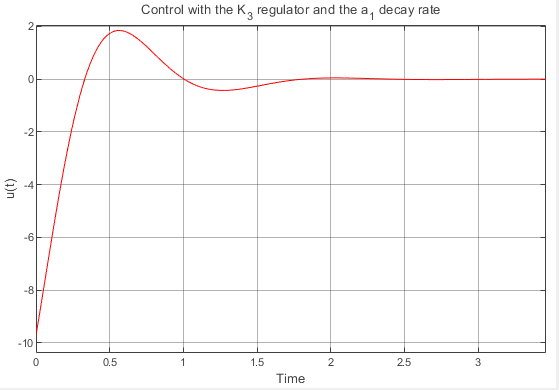
\includegraphics{1task_K3a1_u.png}
        \captionsetup{skip=0pt}
        \caption{График $u(t)$ для $\alpha_1=2$ при $K_{3\,\alpha_1}$}
        \label{fig:1task_K3a1_u}
    \end{figure}
    \begin{figure}[H]
        \centering
        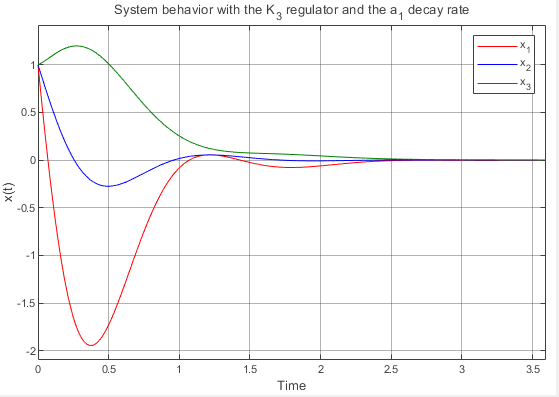
\includegraphics{1task_K3a1_x.png}
        \captionsetup{skip=0pt}
        \caption{График $x(t)$ для $\alpha_1=2$ при $K_{3\,\alpha_1}$}
        \label{fig:1task_K3a1_x}
    \end{figure}
    \newpage
    \vspace*{0.01mm}
    \begin{figure}[H]
        \centering
        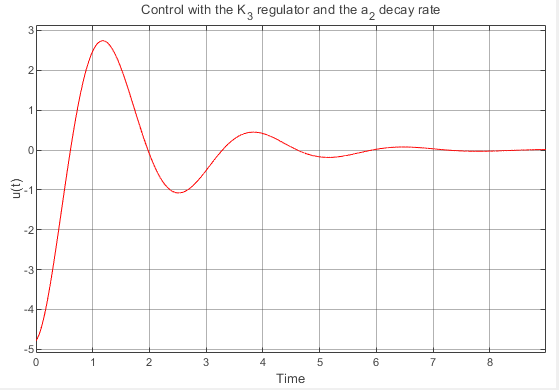
\includegraphics{1task_K3a2_u.png}
        \captionsetup{skip=0pt}
        \caption{График $u(t)$ для $\alpha_2=0.1$ при $K_{3\,\alpha_2}$}
        \label{fig:1task_K3a2_u}
    \end{figure}
    \begin{figure}[H]
        \centering
        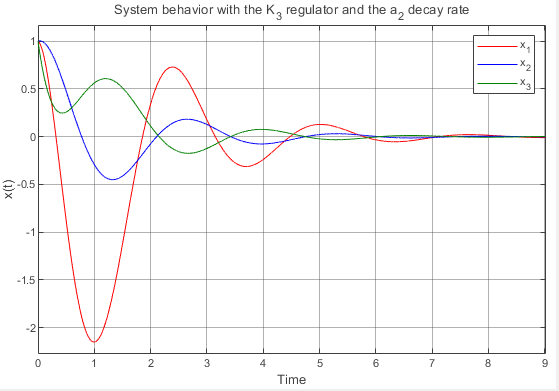
\includegraphics{1task_K3a2_x.png}
        \captionsetup{skip=0pt}
        \caption{График $x(t)$ для $\alpha_1=0.1$ при $K_{3\,\alpha_2}$}
        \label{fig:1task_K3a2_x}
    \end{figure}
    \newpage
    \vspace*{0.01mm}
    \begin{figure}[H]
        \centering
        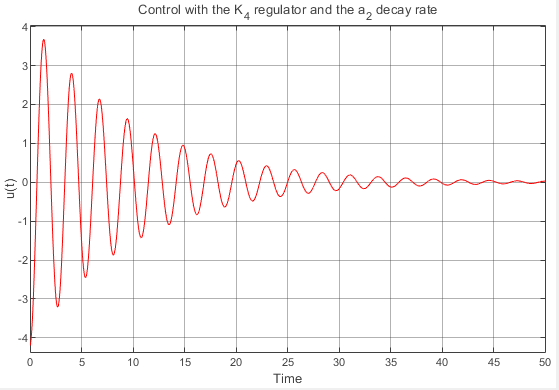
\includegraphics{1task_K4a2_u.png}
        \captionsetup{skip=0pt}
        \caption{График $u(t)$ для $\alpha_2=0.1$ при $K_{4\,\alpha_2}$}
        \label{fig:1task_K4a2_u}
    \end{figure}
    \begin{figure}[H]
        \centering
        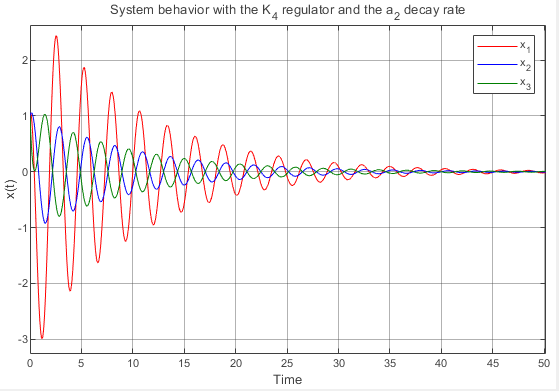
\includegraphics{1task_K4a2_x.png}
        \captionsetup{skip=0pt}
        \caption{График $x(t)$ для $\alpha_1=0.1$ при $K_{4\,\alpha_2}$}
        \label{fig:1task_K4a2_x}
    \end{figure}


    \subsection{Сопоставление результатов для дополнительного пункта}
    Видим, что в случаях с $K_4$ система приобретает больше осцилляций,
    чем с $K_3$ (сравн. рис. \ref{fig:1task_K2a1_x}, \ref{fig:1task_K3a1_x} и \ref{fig:1task_K4a2_x}, \ref{fig:1task_K3a2_x}).
    Время схождения системы к нулю быстрее с $K_3$, однако с $K_4$ требуется меньше управления. В общем графики
    почти совпадают с результатами для $K_{1,2}$ (в случае $K_{4\,\alpha_1}$ результаты полностью совпали с $K_{2\,\alpha_1}$). Таким образом,
    можно предположить, что синтез регулятора через матричное уравнение Риккати почти решает задачу минимизации управления.


    \subsection{Вывод}
    В данном задании был исследован синтез регулятора через матричное неравенство типа Ляпунова и
    матричное уравнение типа Риккати. Были получены графики, подтверждающие корректность расчетов и рассуждений.
    Удалось получить желаемую степень устойчивости с помощью неограниченного и минимального управлений. Результат решения через Риккати
    напоминает результат решения задачи минимизации управления.


    \section{Задание 2. Управление по выходу с заданной степенью устойчивости}
    Рассмотрим систему
    $$
    \begin{cases}
        \dot{x}=Ax+Bu,\\
        y=Cx,
    \end{cases}\ A=\begin{bmatrix}
        2 &0 &-4 &2\\
        0 &2 &-2 &4\\
        -4 &-2 &2 &0\\
        2 &4 &0 &2
    \end{bmatrix},\ B=\begin{bmatrix}
        2\\4\\6\\8
    \end{bmatrix},\ C=\begin{bmatrix}
        -2 &2 &2 &2\\
        2 &0 &0 &2
    \end{bmatrix};
    $$


    \subsection{Управляемость, стабилизируемость, наблюдаемость и обнаруживаемость}
    Найдем собственные числа матрицы $A$. Программа для вычислений в \texttt{MATLAB} представлена на листинге \ref{task2code} в приложении Б
    $$
    \sigma\left( A \right)=\left\{ 0,-4,4,8 \right\}
    $$
    Собственное число $\lambda_2=-4$ асимптотически устойчивое, может быть неуправляемым и/или
    ненаблюдаемым. $\lambda_1=0$ устойчиво, но не асимптотически. Числа $\lambda_{3,4}>0$ неустойчивые,
    нужна управляемость и наблюдаемость.
    Аналогично первому заданию найдем жорданово разложение матрицы $A$ и матрицы $B,C$
    в базисе ее собственных векторов
    $$
    A=PJP^{-1}=\begin{bmatrix}
    1    &-1     &1    &-1\\
    -1    &-1     &1     &1\\
     1    &-1    &-1     &1\\
     1     &1     &1     &1
    \end{bmatrix}\begin{bmatrix}
    0     &0     &0     &0\\
    0    &-4     &0     &0\\
    0     &0     &8     &0\\
    0     &0     &0     &4
    \end{bmatrix}\begin{bmatrix}
    0.25   &-0.25    &0.25    &0.25\\
   -0.25   &-0.25   &-0.25    &0.25\\
    0.25    &0.25   &-0.25    &0.25\\
   -0.25    &0.25    &0.25    &0.25
    \end{bmatrix},
    $$
    $$
    B_J=\begin{bmatrix}
        3\\
    -1\\
     2\\
     4
    \end{bmatrix},\ C_J=\begin{bmatrix}
        0     &0     &0     &8\\
     4     &0     &4     &0
    \end{bmatrix};
    $$
    Все жордановы клетки относятся к различным собственным числам.
    В матрице $B_J$ отсутствуют нулевые элементы -- все собственные числа управляемые. Следовательно,
    система полностью управляема и стабилизируема. В матрице $C_J$ второй столбец нулевой -- асимптотически устойчивое число
    $-4$ является ненаблюдаемым. Система не полностью наблюдаема, но обнаруживаема.

    
    \subsection{Степень устойчивости}
    Так как система полностью управляема, то с помощью регулятора вида $u=Kx$ можно добиться
    любой желаемой степени устойчивости.


    \subsection{Степень сходимости}
    Так как система не полностью наблюдаема, то от наблюдателя полной размерности не получится
    добиться любой желаемой степени сходимости. Максимально возможная $\alpha_L=4$, так как
    ненаблюдаемое собственное число $\lambda_2=-4$.


    \subsection{Схема моделирования системы, замкнутой регулятором, состоящим из наблюдателя состояния и закона управления}
    Построим схему моделирования системы, замкнутой регулятором, состоящим из наблюдателя состояния
    $\dot{\hat{x}}=A\hat{x}+Bu+L\left( C\hat{x}-y \right)$ и закона управления $u=K\hat{x},$ используя \texttt{SIMULINK}.
    Данная схема позволяет построить график $u(t)$ и покомпонентно графики $e(t),\left(x(t),\hat{x}(t)\right)$
    \begin{figure}[H]
        \centering
        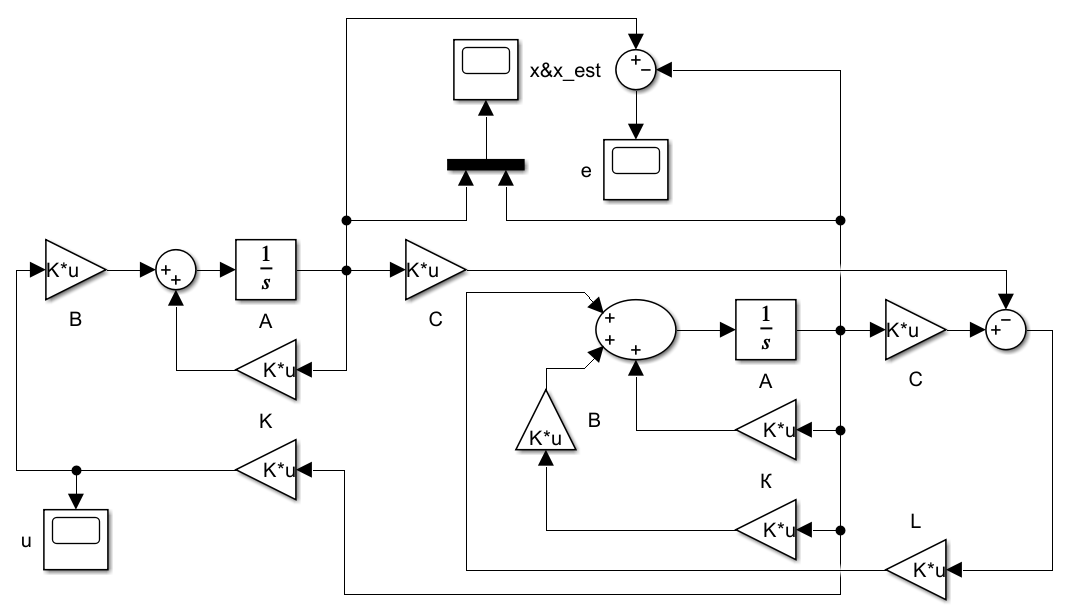
\includegraphics[scale=0.5]{scheme_task2.png}
        \captionsetup{skip=0pt}
        \caption{Схема моделирования системы, замкнутой регулятором, состоящим из наблюдателя состояния и закона управления}
        \label{fig:scheme_task2}
    \end{figure}


    \subsection{Желаемые значения степени устойчивости и сходимости}
    Зададимся парой значений $\alpha>0$, которые будут сильно отличаться, при этом
    одно из них будет максимально возможным, другое достижимым
    \begin{align*}
        &\alpha_1=4,\\
        &\alpha_2=1;
    \end{align*}


    \subsection{Наборы значений желаемой степени устойчивости и сходимости}
    Составим 3 набора значений желаемых степеней устойчивости $\alpha_K$ и сходимости $\alpha_L$
    \begin{align*}
        &\alpha_K=\alpha_L=4\\
        &\alpha_K>\alpha_L\Leftrightarrow 4>1\\
        &\alpha_K<\alpha_L\Leftrightarrow 1<4
    \end{align*}


    \subsection{Синтез регулятора}
    Процесс вычислений аналогичен первому заданию. Используем метод уравнений Риккати и \texttt{MATLAB}.
    Будем подбирать матрицу $Q$, при которой отклонения собственных чисел спектра замкнутой системы
    от желаемой степени устойчивости будут минимизированы.


    Вычислим $K_{\alpha_1}$ для $\alpha_K=4$ при $Q=0,\,\nu=2,\,R=1$
    $$
    K_{\alpha_1}=
    \begin{bmatrix}
        -24.5000   &-5.5000   &20.5000   &-9.5000
    \end{bmatrix}
    $$
    Проверим собственные числа замкнутой системы $A+BK_{\alpha_1}$
    $$
    \sigma\left( A+BK_{\alpha_1} \right)=\left\{ -4,-4,-4.0000\pm13.2665i \right\}
    $$
    Действительные части всех собственных чисел совпадают с желаемой степенью устойчивости $\alpha_K=4$.
    Регулятор синтезирован корректно.


    Вычислим $K_{\alpha_2}$ для $\alpha_K=1$ при $Q=0.000001\cdot I,\,\nu=2,\,R=1$:
    $$
    K_{\alpha_2}=
    \begin{bmatrix}
        -6.7188   &-3.1250    &6.4063   &-3.4375
    \end{bmatrix}
    $$
    Выполним аналогичную проверку замкнутой системы
    $$
    \sigma\left( A+BK_{\alpha_2} \right)=\left\{ -4,-1,-1.0000 \pm 7.6812i \right\}
    $$
    Действительные части трех собственных чисел совпадают с желаемой степенью устойчивости $\alpha_K=1$.
    Одно из чисел всегда остается равным $-4$. Можем сделать вывод, что регулятор синтезирован корректно.


    \subsection{Синтез наблюдателя}
    Матрицы наблюдателя $L$ будем искать с помощью матричных неравенств
    $$
    Q\succ0,\ A^TQ+QA+2\alpha Q+C^TY^T+YC\prec 0,\ L=Q^{-1}Y;
    $$
    Алгоритм минимизации аналогичен первому заданию, разве что $\gamma$ уже будет не скаляр,
    а матрица размера $2\times2$. Минимизировать будем ее норму. Решаем через \texttt{cvx}.
    Так как размерность выхода $C$ другая, то и $Y$ станет другой размерности -- $4\times2$.
    Для вычисления также понадобятся начальные условия для системы и наблюдателя
    $$
    x(0)=\begin{bmatrix}
        1\\1\\1\\1
    \end{bmatrix},\ \hat{x}(0)=\begin{bmatrix}
        0\\0\\0\\0
    \end{bmatrix};
    $$


    Вычислим $L_{\alpha_1}$ для $\alpha_L=4$
    $$
    L_{\alpha_1}=\begin{bmatrix}
        2.2450   &-4.0000\\
        -0.1281   &-8.0000\\
        -2.1222    &8.0000\\
        -0.0089   &-4.0000
    \end{bmatrix}
    $$
    Проверим собственные числа замкнутой системы $A+BL_{\alpha_1}$
    $$
    \sigma\left( A+BL_{\alpha_1} \right)=\left\{ -5.0084, -4, -4.0000 \pm 6.9282i \right\}
    $$
    Действительные части собственных чисел близки к желаемой степени сходимости $\alpha_L=4$. Наблюдатель синтезирован корректно.


    Вычислим $L_{\alpha_2}$ для $\alpha_L=1$
    $$
    L_{\alpha_2}=\begin{bmatrix}
        1.3693   &-2.5000\\
   -0.0350   &-3.1253\\
   -1.3365    &3.1273\\
    0.0021   &-2.5020
    \end{bmatrix}
    $$
    Выполним аналогичную проверку замкнутой системы
    $$
    \sigma\left( A+BL_{\alpha_2} \right)=\left\{ -4, -1.4772, -1.0020 \pm 3.0000i \right\}
    $$
    Действительные части собственных чисел близки к желаемой степени сходимости $\alpha_L=1$.
    Наблюдаем в спектре неуправляемое собственное число $\lambda_1=-4$ матрицы $A$.
    Можем сделать вывод, что наблюдатель синтезирован корректно.


    \subsection{Компьютерное моделирование}
    Выполним компьютерное моделирование с начальными условиями системы
    $$
    x(0)=\begin{bmatrix}
        1\\1\\1\\1
    \end{bmatrix}
    $$
    и наблюдателя
    $$
    \hat{x}(0)=\begin{bmatrix}
        0\\0\\0\\0
    \end{bmatrix}
    $$
    Построим графики формируемого управления $u(t)$, сравнительные графики $x(t)$ и $\hat{x}(t)$ (покомпонентно),
    а также график ошибки наблюдателя $e(t)=x(t)-\hat{x}(t)$. Для построения пользуемся схемой, представленной на рис. \ref{fig:scheme_task2}.


    Далее расположены перечисленные графики на рис. \ref{2task_aKeqaL_x1}--\ref{2task_aKlaL_u}

    
    % 963,257,718,369
    \newpage
    \vspace*{20mm}
    \begin{figure}[H]
        \centering
        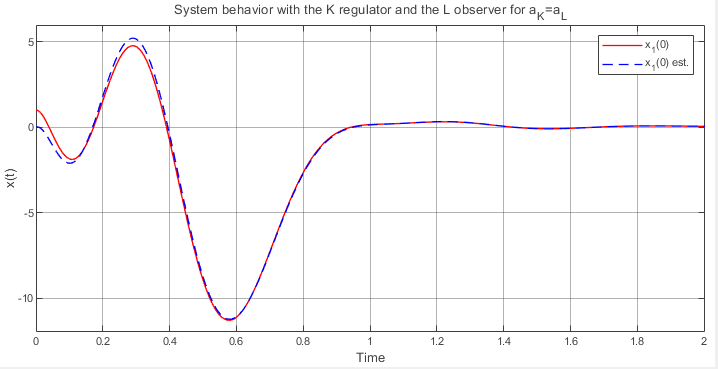
\includegraphics[scale=0.8]{2task_aK=aL_x1.png}
        \captionsetup{skip=0pt}
        \caption{Графики $x_1(t),\hat{x}_1(t)$ для $\alpha_K=\alpha_L=4$}
        \label{2task_aKeqaL_x1}
    \end{figure}
    \begin{figure}[H]
        \centering
        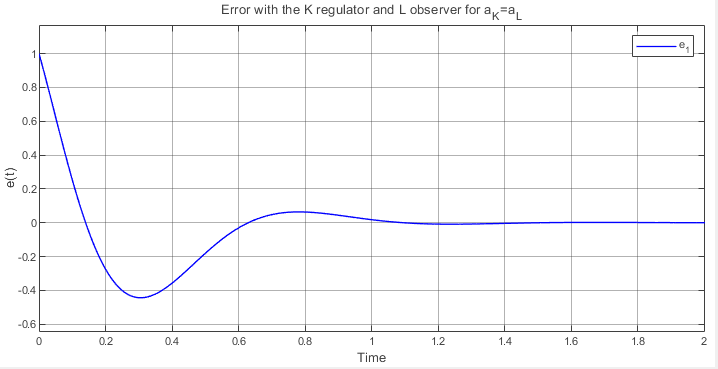
\includegraphics[scale=0.8]{2task_aK=aL_e1.png}
        \captionsetup{skip=0pt}
        \caption{График $e_1(t)$ для $\alpha_K=\alpha_L=4$}
        \label{2task_aKeqaL_e1}
    \end{figure}
    \newpage
    \vspace*{20mm}
    \begin{figure}[H]
        \centering
        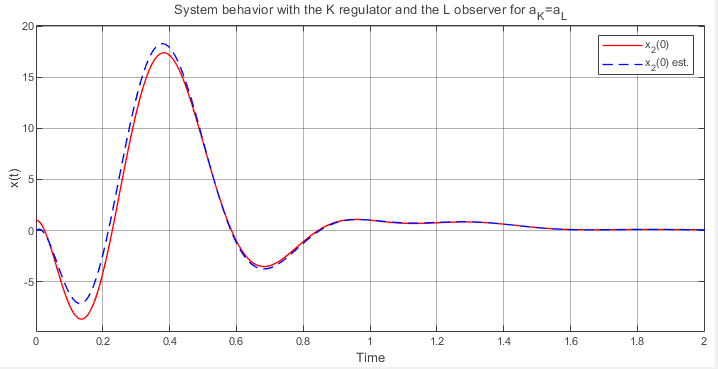
\includegraphics[scale=0.8]{2task_aK=aL_x2.png}
        \captionsetup{skip=0pt}
        \caption{Графики $x_2(t),\hat{x}_2(t)$ для $\alpha_K=\alpha_L=4$}
        \label{2task_aKeqaL_x2}
    \end{figure}
    \begin{figure}[H]
        \centering
        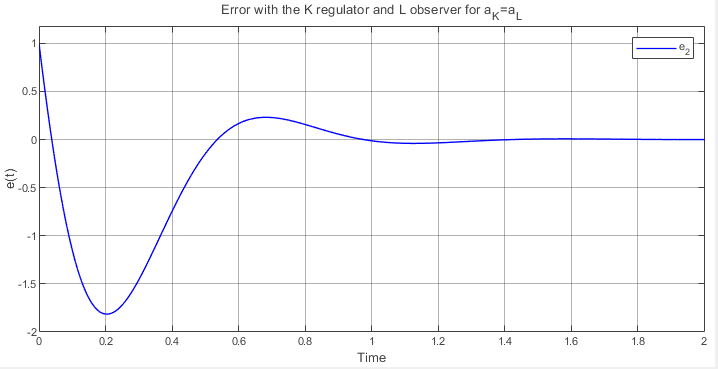
\includegraphics[scale=0.8]{2task_aK=aL_e2.png}
        \captionsetup{skip=0pt}
        \caption{График $e_2(t)$ для $\alpha_K=\alpha_L=4$}
        \label{2task_aKeqaL_e2}
    \end{figure}
    \newpage
    \vspace*{20mm}
    \begin{figure}[H]
        \centering
        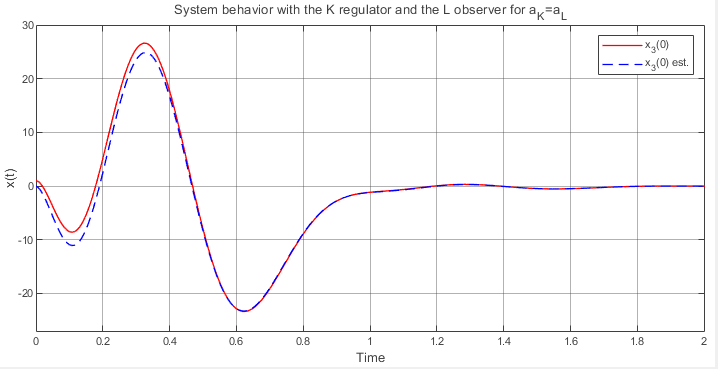
\includegraphics[scale=0.8]{2task_aK=aL_x3.png}
        \captionsetup{skip=0pt}
        \caption{Графики $x_3(t),\hat{x}_3(t)$ для $\alpha_K=\alpha_L=4$}
        \label{2task_aKeqaL_x3}
    \end{figure}
    \begin{figure}[H]
        \centering
        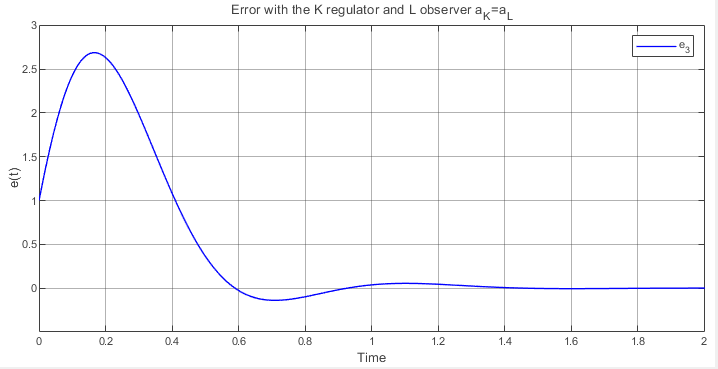
\includegraphics[scale=0.8]{2task_aK=aL_e3.png}
        \captionsetup{skip=0pt}
        \caption{График $e_3(t)$ для $\alpha_K=\alpha_L=4$}
        \label{2task_aKeqaL_e3}
    \end{figure}
    \newpage
    \vspace*{20mm}
    \begin{figure}[H]
        \centering
        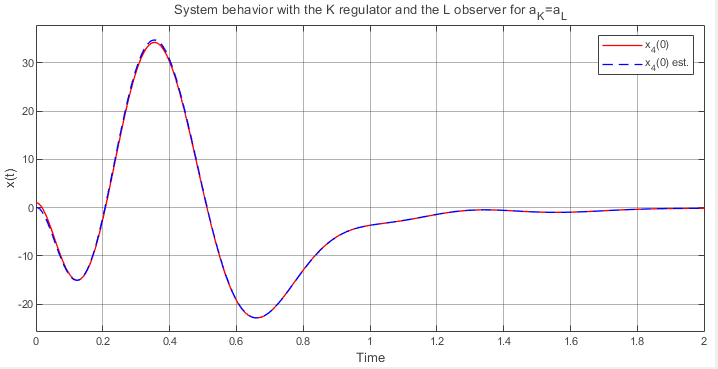
\includegraphics[scale=0.8]{2task_aK=aL_x4.png}
        \captionsetup{skip=0pt}
        \caption{Графики $x_4(t),\hat{x}_4(t)$ для $\alpha_K=\alpha_L=4$}
        \label{2task_aKeqaL_x4}
    \end{figure}
    \begin{figure}[H]
        \centering
        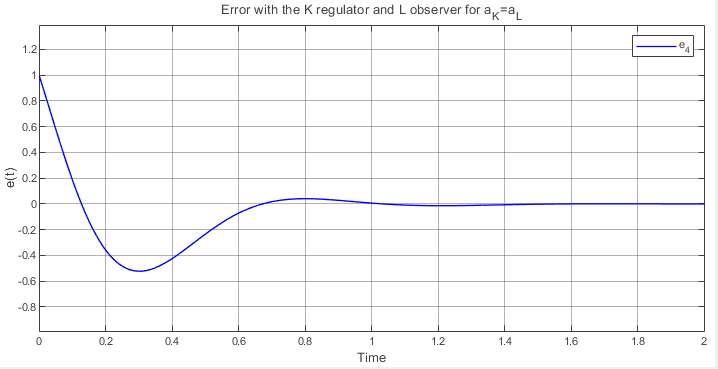
\includegraphics[scale=0.8]{2task_aK=aL_e4.png}
        \captionsetup{skip=0pt}
        \caption{График $e_4(t)$ для $\alpha_K=\alpha_L=4$}
        \label{2task_aKeqaL_e4}
    \end{figure}
    \newpage
    \vspace*{20mm}
    \begin{figure}[H]
        \centering
        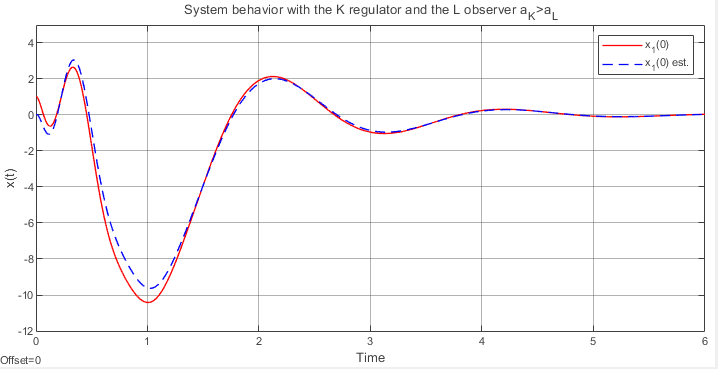
\includegraphics[scale=0.8]{2task_aKgaL_x1.png}
        \captionsetup{skip=0pt}
        \caption{Графики $x_1(t),\hat{x}_1(t)$ для $\alpha_K>\alpha_L\Leftrightarrow4>1$}
        \label{2task_aKgaL_x1}
    \end{figure}
    \begin{figure}[H]
        \centering
        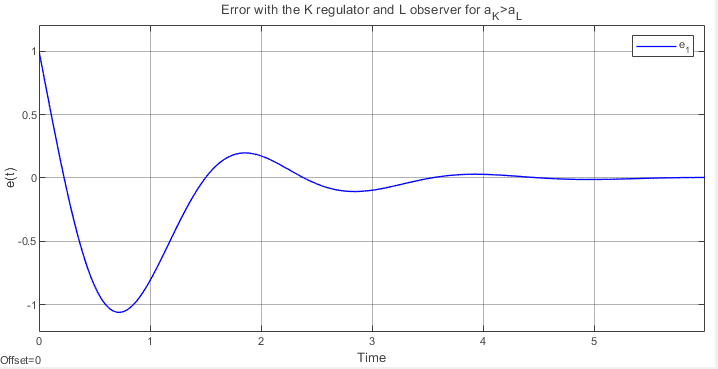
\includegraphics[scale=0.8]{2task_aKgaL_e1.png}
        \captionsetup{skip=0pt}
        \caption{График $e_1(t)$ для $\alpha_K>\alpha_L\Leftrightarrow4>1$}
        \label{2task_aKgaL_e1}
    \end{figure}
    \newpage
    \vspace*{20mm}
    \begin{figure}[H]
        \centering
        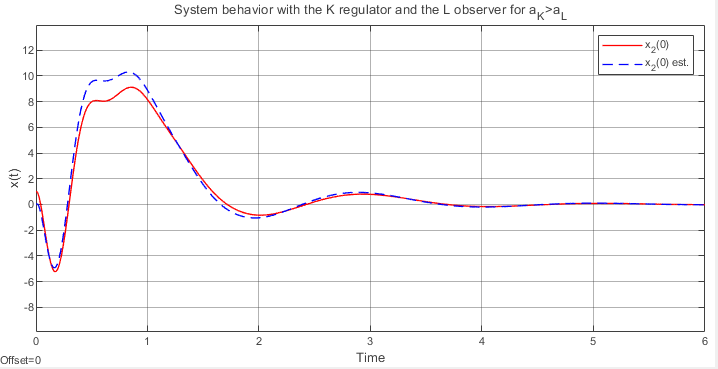
\includegraphics[scale=0.8]{2task_aKgaL_x2.png}
        \captionsetup{skip=0pt}
        \caption{Графики $x_2(t),\hat{x}_2(t)$ для $\alpha_K>\alpha_L\Leftrightarrow4>1$}
        \label{2task_aKgaL_x2}
    \end{figure}
    \begin{figure}[H]
        \centering
        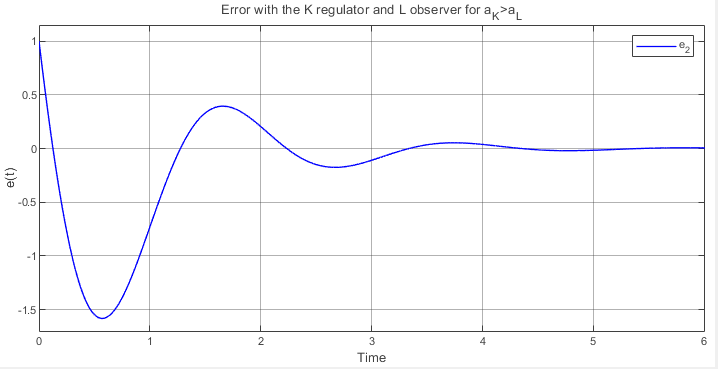
\includegraphics[scale=0.8]{2task_aKgaL_e2.png}
        \captionsetup{skip=0pt}
        \caption{График $e_2(t)$ для $\alpha_K>\alpha_L\Leftrightarrow4>1$}
        \label{2task_aKgaL_e2}
    \end{figure}
    \newpage
    \vspace*{20mm}
    \begin{figure}[H]
        \centering
        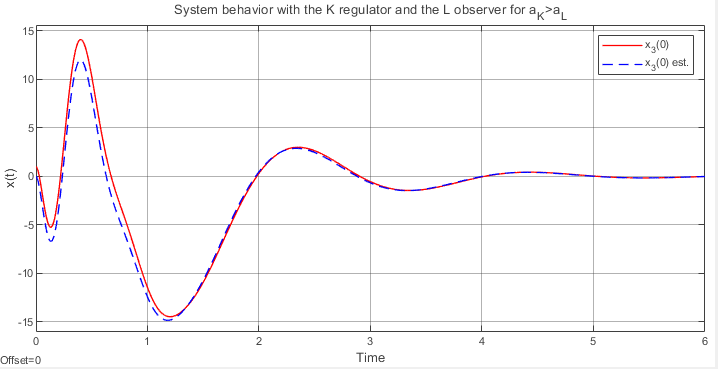
\includegraphics[scale=0.8]{2task_aKgaL_x3.png}
        \captionsetup{skip=0pt}
        \caption{Графики $x_3(t),\hat{x}_3(t)$ для $\alpha_K>\alpha_L\Leftrightarrow4>1$}
        \label{2task_aKgaL_x3}
    \end{figure}
    \begin{figure}[H]
        \centering
        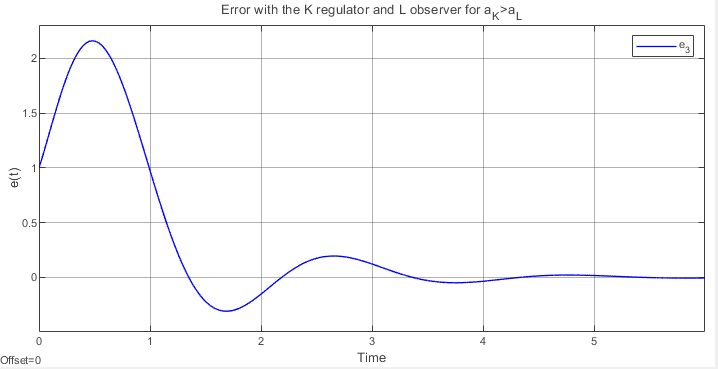
\includegraphics[scale=0.8]{2task_aKgaL_e3.png}
        \captionsetup{skip=0pt}
        \caption{График $e_3(t)$ для $\alpha_K>\alpha_L\Leftrightarrow4>1$}
        \label{2task_aKgaL_e3}
    \end{figure}
    \newpage
    \vspace*{20mm}
    \begin{figure}[H]
        \centering
        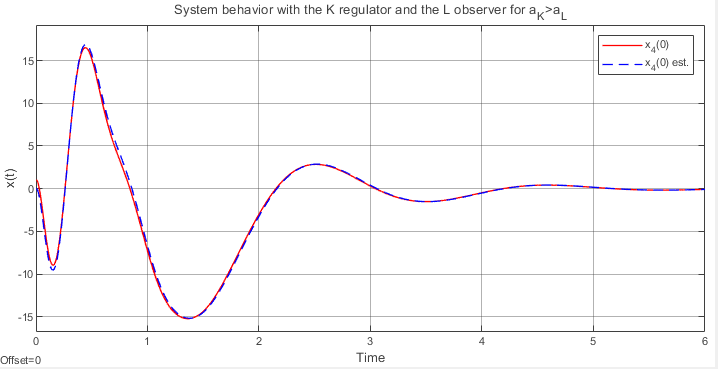
\includegraphics[scale=0.8]{2task_aKgaL_x4.png}
        \captionsetup{skip=0pt}
        \caption{Графики $x_4(t),\hat{x}_4(t)$ для $\alpha_K>\alpha_L\Leftrightarrow4>1$}
        \label{2task_aKgaL_x4}
    \end{figure}
    \begin{figure}[H]
        \centering
        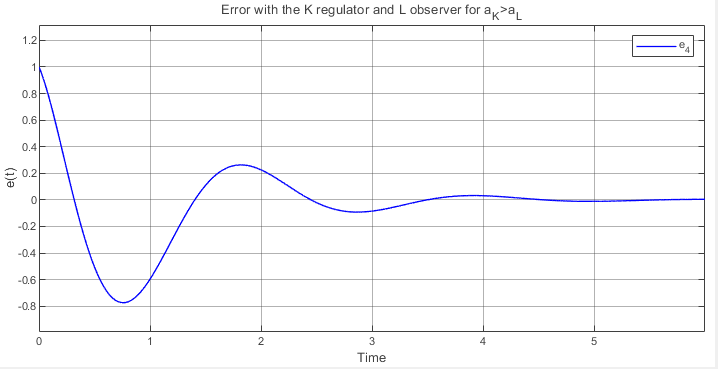
\includegraphics[scale=0.8]{2task_aKgaL_e4.png}
        \captionsetup{skip=0pt}
        \caption{График $e_4(t)$ для $\alpha_K>\alpha_L\Leftrightarrow4>1$}
        \label{2task_aKgaL_e4}
    \end{figure}
    \newpage
    \vspace*{20mm}
    \begin{figure}[H]
        \centering
        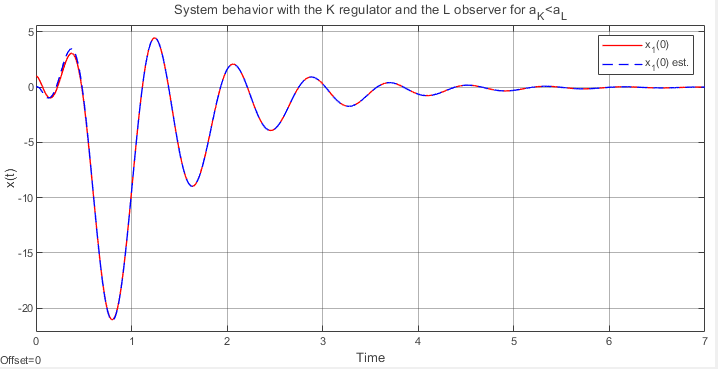
\includegraphics[scale=0.8]{2task_aKlaL_x1.png}
        \captionsetup{skip=0pt}
        \caption{Графики $x_1(t),\hat{x}_1(t)$ для $\alpha_K<\alpha_L\Leftrightarrow1<4$}
        \label{2task_aKlaL_x1}
    \end{figure}
    \begin{figure}[H]
        \centering
        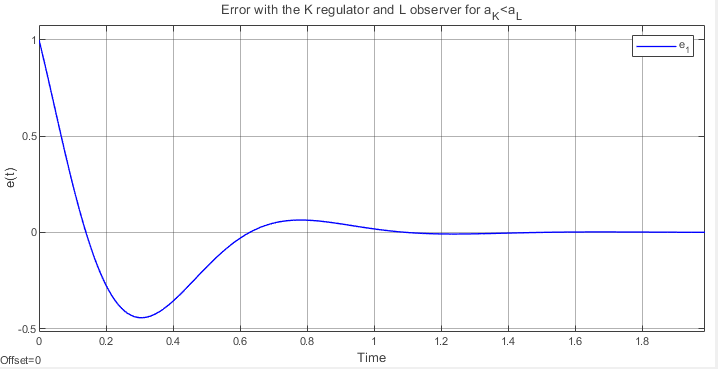
\includegraphics[scale=0.8]{2task_aKlaL_e1.png}
        \captionsetup{skip=0pt}
        \caption{График $e_1(t)$ для $\alpha_K<\alpha_L\Leftrightarrow1<4$}
        \label{2task_aKlaL_e1}
    \end{figure}
    \newpage
    \vspace*{20mm}
    \begin{figure}[H]
        \centering
        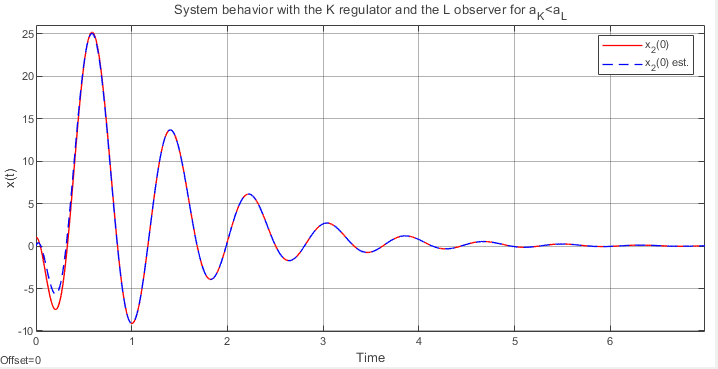
\includegraphics[scale=0.8]{2task_aKlaL_x2.png}
        \captionsetup{skip=0pt}
        \caption{Графики $x_2(t),\hat{x}_2(t)$ для $\alpha_K<\alpha_L\Leftrightarrow1<4$}
        \label{2task_aKlaL_x2}
    \end{figure}
    \begin{figure}[H]
        \centering
        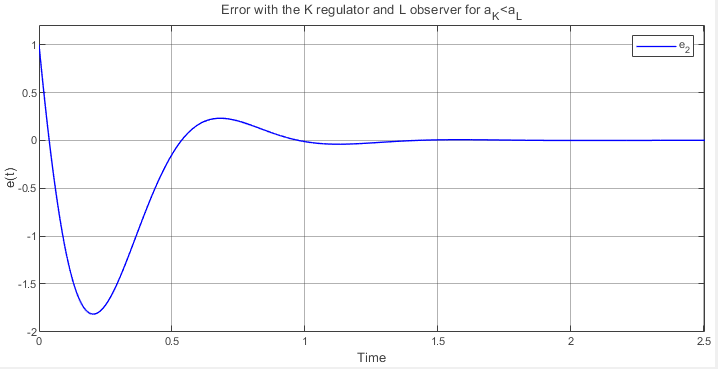
\includegraphics[scale=0.8]{2task_aKlaL_e2.png}
        \captionsetup{skip=0pt}
        \caption{График $e_2(t)$ для $\alpha_K<\alpha_L\Leftrightarrow1<4$}
        \label{2task_aKlaL_e2}
    \end{figure}
    \newpage
    \vspace*{20mm}
    \begin{figure}[H]
        \centering
        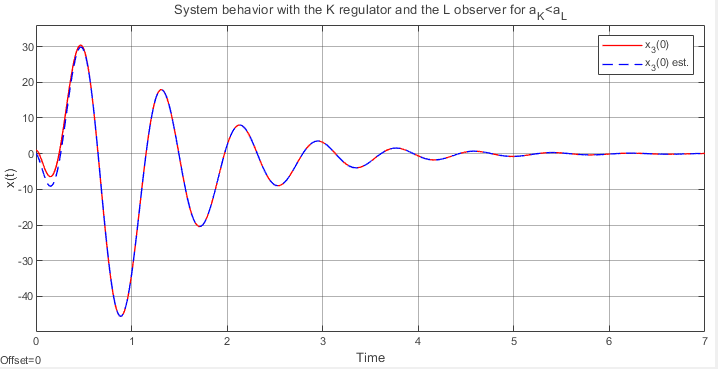
\includegraphics[scale=0.8]{2task_aKlaL_x3.png}
        \captionsetup{skip=0pt}
        \caption{Графики $x_3(t),\hat{x}_3(t)$ для $\alpha_K<\alpha_L\Leftrightarrow1<4$}
        \label{2task_aKlaL_x3}
    \end{figure}
    \begin{figure}[H]
        \centering
        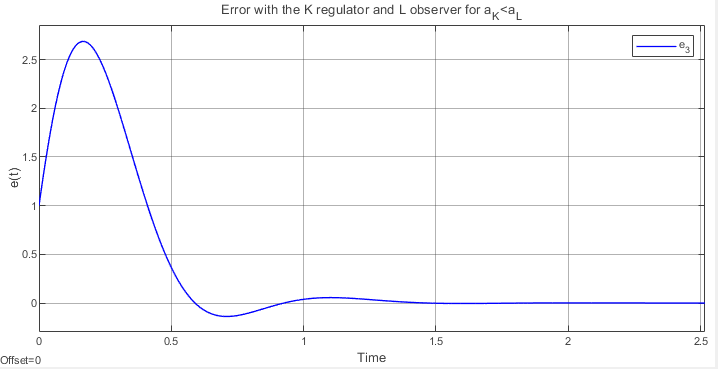
\includegraphics[scale=0.8]{2task_aKlaL_e3.png}
        \captionsetup{skip=0pt}
        \caption{График $e_3(t)$ для $\alpha_K<\alpha_L\Leftrightarrow1<4$}
        \label{2task_aKlaL_e3}
    \end{figure}
    \newpage
    \vspace*{20mm}
    \begin{figure}[H]
        \centering
        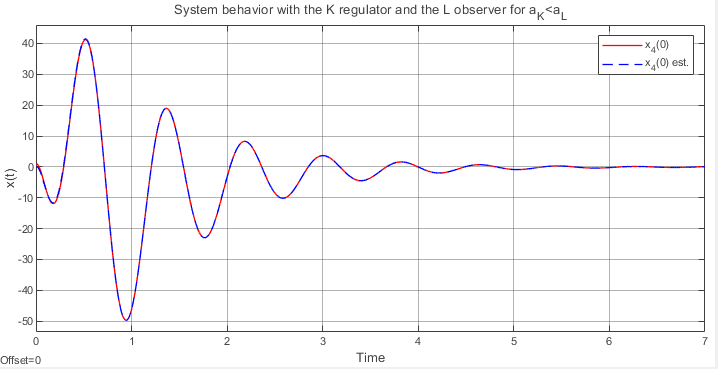
\includegraphics[scale=0.8]{2task_aKlaL_x4.png}
        \captionsetup{skip=0pt}
        \caption{Графики $x_4(t),\hat{x}_4(t)$ для $\alpha_K<\alpha_L\Leftrightarrow1<4$}
        \label{2task_aKlaL_x4}
    \end{figure}
    \begin{figure}[H]
        \centering
        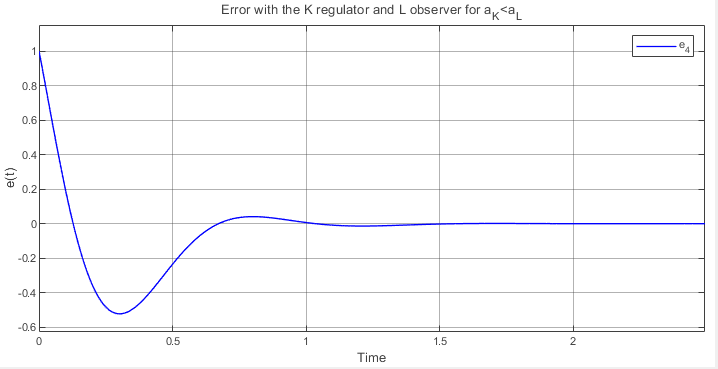
\includegraphics[scale=0.8]{2task_aKlaL_e4.png}
        \captionsetup{skip=0pt}
        \caption{График $e_4(t)$ для $\alpha_K<\alpha_L\Leftrightarrow1<4$}
        \label{2task_aKlaL_e4}
    \end{figure}
    \newpage
    \begin{figure}[H]
        \centering
        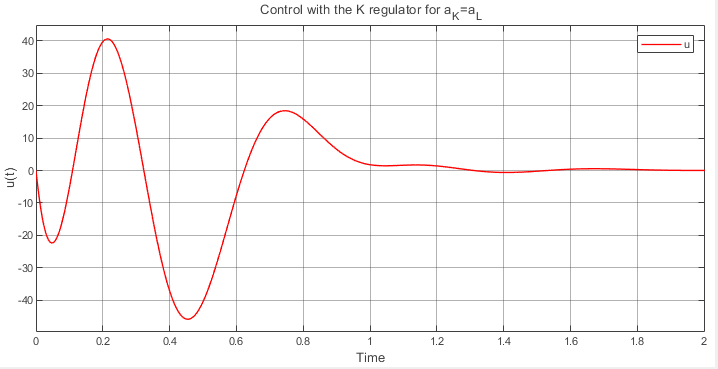
\includegraphics[scale=0.74]{2task_aK=aL_u.png}
        \captionsetup{skip=0pt}
        \caption{График $u(t)$ для $\alpha_K=\alpha_L=4$}
        \label{2task_aKeqaL_u}
    \end{figure}
    \begin{figure}[H]
        \centering
        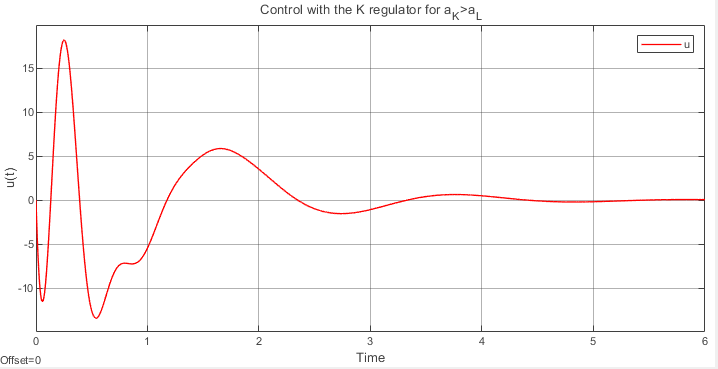
\includegraphics[scale=0.74]{2task_aKgaL_u.png}
        \captionsetup{skip=0pt}
        \caption{График $u(t)$ для $\alpha_K>\alpha_L\Leftrightarrow4>1$}
        \label{2task_aKgaL_u}
    \end{figure}
    \begin{figure}[H]
        \centering
        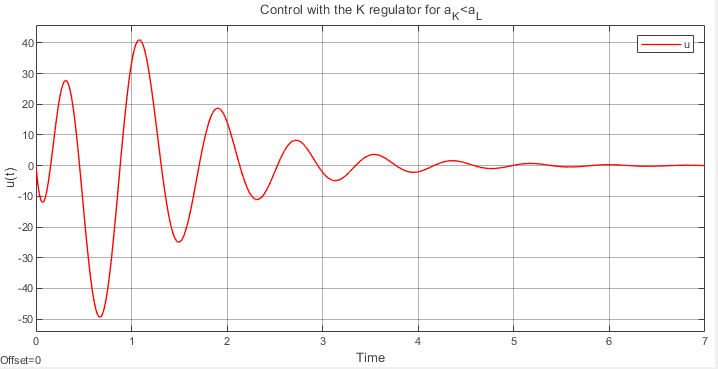
\includegraphics[scale=0.74]{2task_aKlaL_u.png}
        \captionsetup{skip=0pt}
        \caption{График $u(t)$ для $\alpha_K<\alpha_L\Leftrightarrow1<4$}
        \label{2task_aKlaL_u}
    \end{figure}
    
    
    \subsection{Сравнение результатов}
    При $\alpha_K<\alpha_L$ система стабилизируется медленнее в сравнении с другими случаями,
    но наблюдатель раньше приходит к истинному состоянию системы (сравн. рис. \ref{2task_aKlaL_x4}, \ref{2task_aKgaL_x4}, \ref{2task_aKeqaL_x4}).
    Быстрее всего система сошлась к нулю при сопоставимых значениях $\alpha_K=\alpha_L$ (сравн. рис. \ref{2task_aKeqaL_x1}, \ref{2task_aKgaL_x1}, \ref{2task_aKlaL_x1}). Меньше всего
    управления потребовалось, когда $\alpha_K>\alpha_L$ (сравн. рис. \ref{2task_aKeqaL_u}, \ref{2task_aKgaL_u}, \ref{2task_aKlaL_u}).
    Медленнее всего наблюдатель сходится к истинным траекториям системы при $\alpha_K>\alpha_L$ (сравн. \ref{2task_aKgaL_x2} с \ref{2task_aKeqaL_x2}, \ref{2task_aKlaL_x2}; \ref{2task_aKgaL_x3} с \ref{2task_aKeqaL_x3}, \ref{2task_aKlaL_x3}).


    \subsection{Вывод}
    В данном задании мы выяснили, что система полностью управляема, стабилизируема, не полностью наблюдаема и обнаруживаема.
    Мы экспериментировали с влиянием регулятора и наблюдателя с различными наборами значений степени устойчивости и сходимости на систему.
    Были получены соответствующие матрицы $K,L$ и проведено компьютерное моделирование. Результаты подтвердили корретность проведенных расчетов.
    По графикам были сделаны выводы об управлении и слежении.


    \section{Задание 3. Регулятор с качественной экспоненциальной устойчивостью}
    Рассмотрим систему
    $$
    \dot{x}=Ax+Bu,\ A=\begin{bmatrix}
        5 &2 &7\\
        2 &1 &2\\
        -2 &-3 &-4
    \end{bmatrix},\ B=\begin{bmatrix}
        3\\1\\-1
    \end{bmatrix};
    $$


    \subsection{Управляемость и стабилизируемость}
    В первом задании мы уже находили собственные числа матрицы $A$. Программа для третьего задания
    находится на листинге \ref{task3code} в приложении В
    $$
    \sigma\left( A \right)=\left\{ -2,2\pm i \right\}
    $$
    Собственное число $\lambda_1=-2$ асимптотически устойчивое, может быть неуправляемым. Комплексная пара неустойчивая,
    нужна управляемость. Найдем матрицу $J_{re}$ из вещественного жорданова разложения матрицы $A=P_{re}J_{re}P_{re}^{-1}$.
    Переведем матрицу $B$ в базис собственных векторов матрицы $A$
    $$
    J_{re}=\begin{bmatrix}
    -2     &0     &0\\
    0     &2     &1\\
    0    &-1     &2
    \end{bmatrix},\ B_{Jre}=\begin{bmatrix}
        0\\
     3\\
    -1
    \end{bmatrix};
    $$
    Все жордановы клетки относятся к различным собственным числам. Число $\lambda_1=-2$ является неуправляемым,
    остальные управляемые (первый элемент $B_{Jre}$ -- ноль). Таким образом, система не полностью управляема,
    но стабилизируема.


    \subsection{Средняя степень устойчивости}
    Зададим следующие параметры: $\beta<0$,
    характеризующий среднее значение поведения
    траекторий ($|\beta|$ как <<средняя степень устойчивости>>),
    и $r>0$, характеризующий разброс поведения траекторий относительно
    среднего значения $\beta$. Будем соблюдать условия
    $$
    \beta+r<0,\ r=\dfrac{|\beta|}{k},\ 1.5\leq k\leq 4;\ |\lambda_{\text{неупр.}}-\beta|\leq r;
    $$
    Пусть
    $$
    \beta=-2,\ k=4\Rightarrow r=\dfrac{|-2|}{4}=0.5;\ \lambda_{\text{неупр.}}=-2\Rightarrow |-2-(-2)|=0\leq r=0.5;
    $$


    \subsection{Наборы параметров Q и R}
    Зададимся четырьмя наборами параметров $Q,R$
    \begin{align*}
        &\circ Q=I,\ R=1;\\
        &\circ Q=I,\ R=0;\\
        &\circ Q=0,\ R=1;\\
        &\circ Q=0,\ R=0;
    \end{align*}


    \subsection{Схема моделирования системы, замкнутой регулятором}
    Схема моделирования системы аналогична первому заданию -- см. рис. \ref{fig:scheme_task1}.


    \subsection{Синтез регулятора}
    Для каждого набора параметров $Q,R$ синтезируем регулятор, обеспечивающий качественную экспоненциальную
    устойчивость при помощи матричного уравнения типа Риккати
    $$
    \left( A-BK-\beta I \right)^TP\left( A-BK-\beta I \right)-r^2P=-Q,
    $$
    $$K=-\left( R+B^TPB \right)^{-1}B^TP\left( A-\beta I \right);
    $$
    Пользуемся \texttt{vpasolve()} в \texttt{MATLAB} и рассчитываем на элемент случайности.
    

    Найдем $K_1$ при $Q=I,\ R=1$
    $$
    K_1=\begin{bmatrix}
        -1.8110966785064287110220433888041\\-4.3160849593283698027780387510567\\-1.8110966785064287110220433888041
    \end{bmatrix}^T
    $$
    Проверим собственные числа замкнутой системы $A+BK_1$
    $$
    \sigma\left( A+BK_1 \right)=$$
    $$
    \left\{ -2,-1.9691391581706136124110627643325 \pm 0.072704192232709769030434861420894i \right\}
    $$
    Действительные части собственных чисел отрицательны, похоже на правду. Выведем их на комплексную плоскость,
    чтобы проверить, находятся ли они в пределах круга с центром в точке $\left( \beta;0 \right)$ и радиусом $r$.
    Результат см. рис. \ref{3task_eig_QI_R1}
    \begin{figure}[H]
        \centering
        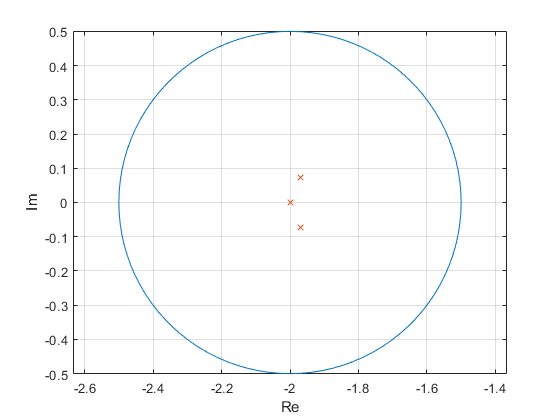
\includegraphics[scale=0.75]{3task_eig_QI_R1.png}
        \captionsetup{skip=0pt}
        \caption{Проверка собственных чисел з. с. $\left(A+BK_1\right)$ при $Q=I,\ R=1$}
        \label{3task_eig_QI_R1}
    \end{figure}
    \noindent Собственные числа находятся внутри круга, следовательно, регулятор синтезирован корректно.


    Повторим шаги для $K_2$ при $Q=I,\ R=0$
    $$
    K_2=\begin{bmatrix}
        -1.8117543951362541390851582228351\\-4.3177192340462210264038924401546\\-1.8117543951362541390851582228351
    \end{bmatrix}^T
    $$
    Проверка $\sigma\left( A+BK_2  \right)$
    $$
    \left\{ -2, -2, -1.9412280243187293045742088858247 \right\}
    $$
    Отрицательные числа -- похоже на правду. Проверим графиком (см. рис. \ref{3task_eig_QI_R0})
    \begin{figure}[H]
        \centering
        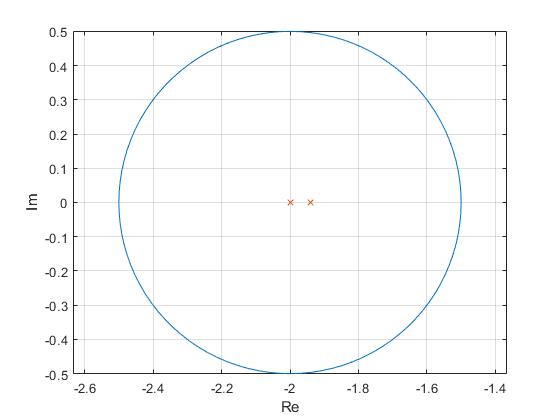
\includegraphics[scale=0.75]{3task_eig_QI_R0.png}
        \captionsetup{skip=0pt}
        \caption{Проверка собственных чисел з. с. $\left(A+BK_2\right)$ при $Q=I,\ R=0$}
        \label{3task_eig_QI_R0}
    \end{figure}
    \noindent Собственные числа находятся внутри круга, следовательно, регулятор синтезирован корректно.


    Найдем $K_3$ при $Q=0,\ R=1$
    $$
    K_3=\begin{bmatrix}
        -1.85 &-4.3 &-1.85
    \end{bmatrix}
    $$
    Проверка собственных чисел замкнутой системы $A+BK_3$
    $$
    \sigma\left( A+BK_3 \right)=\left\{ -2.5, -2, -1.5 \right\}
    $$
    Собственные числа отрицательные -- похоже на правду. Проверим графиком (см. рис. \ref{3task_eig_Q0_R1})
    \begin{figure}[H]
        \centering
        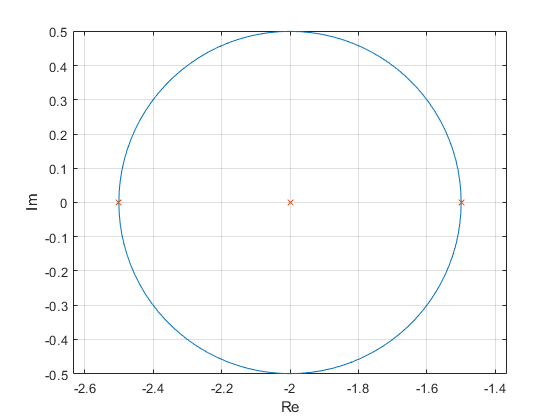
\includegraphics[scale=0.75]{3task_eig_Q0_R1.png}
        \captionsetup{skip=0pt}
        \caption{Проверка собственных чисел з. с. $\left(A+BK_3\right)$ при $Q=0,\ R=1$}
        \label{3task_eig_Q0_R1}
    \end{figure}
    \noindent Собственное число $-2$ находится внутри круга, остальные на его границе.
    Следовательно, регулятор синтезирован корректно.


    Повторим для $K_4$ при $Q=0,\ R=0$
    $$
    K_4=\begin{bmatrix}
        -1.8534107402031930333817126269956\\-4.0261248185776487663280116110305\\-1.8534107402031930333817126269956
    \end{bmatrix}^T
    $$
    Проверим $\sigma\left( A+BK_4 \right)$
    $$
    \left\{ -2, -2, -1.7329462989840348330914368650218 \right\}
    $$
    Наблюдаем отрицательные собственные числа -- похоже на правду. Проверим графиком (см. рис. \ref{3task_eig_Q0_R0})
    \begin{figure}[H]
        \centering
        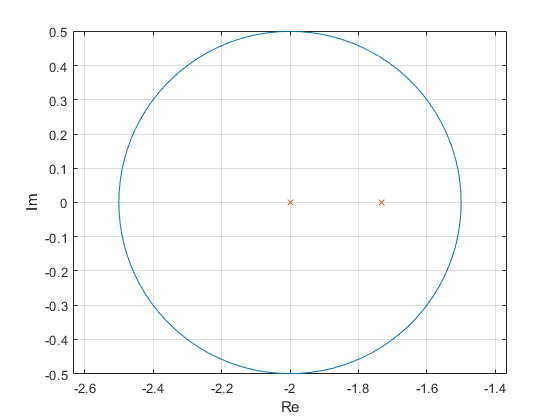
\includegraphics[scale=0.75]{3task_eig_Q0_R0.png}
        \captionsetup{skip=0pt}
        \caption{Проверка собственных чисел з. с. $\left(A+BK_4\right)$ при $Q=0,\ R=0$}
        \label{3task_eig_Q0_R0}
    \end{figure}
    \noindent Собственные числа находятся внутри круга, следовательно, регулятор синтезирован корректно.


    \subsection{Компьютерное моделирование}
    Выполним компьютерное моделирование замкнутых систем по схеме, представленной на рис. \ref{fig:scheme_task1}. Построим
    графики формируемого регуляторами управления $u(t)$ и вектора состояния замкнутых систем $x(t)$
    при начальных условиях $$x(0)=\begin{bmatrix}
        1\\1\\1
    \end{bmatrix}$$
    Результаты представлены далее на рис. \ref{fig:3task_K1_u}--\ref{fig:3task_Ki_u_close}


    \newpage
    \vspace*{0.01mm}
    \begin{figure}[H]
        \centering
        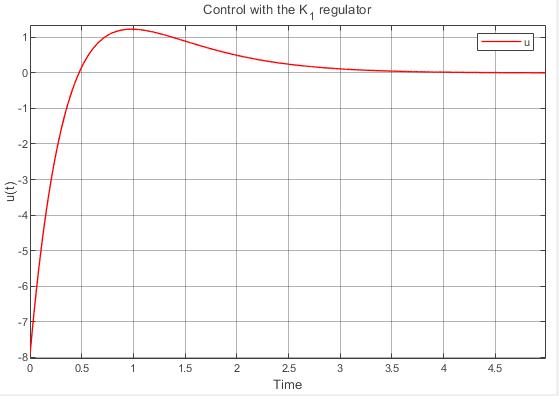
\includegraphics{3task_K1_u.png}
        \captionsetup{skip=0pt}
        \caption{График $u(t)$ при $K_1,\ Q=I,\ R=1$}
        \label{fig:3task_K1_u}
    \end{figure}
    \begin{figure}[H]
        \centering
        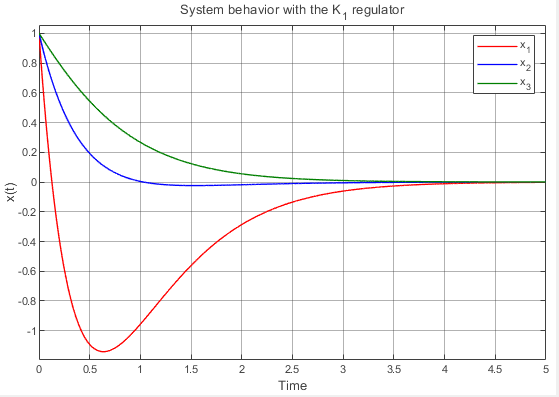
\includegraphics{3task_K1_x.png}
        \captionsetup{skip=0pt}
        \caption{График $x(t)$ при $K_{1},\ Q=I,\ R=1$}
        \label{fig:3task_K1_x}
    \end{figure}
    \newpage
    \vspace*{0.01mm}
    \begin{figure}[H]
        \centering
        \includegraphics{3task_K2_u.png}
        \captionsetup{skip=0pt}
        \caption{График $u(t)$ при $K_2,\ Q=I,\ R=0$}
        \label{fig:3task_K2_u}
    \end{figure}
    \begin{figure}[H]
        \centering
        \includegraphics{3task_K2_x.png}
        \captionsetup{skip=0pt}
        \caption{График $x(t)$ при $K_{2},\ Q=I,\ R=0$}
        \label{fig:3task_K2_x}
    \end{figure}
    \newpage
    \vspace*{0.01mm}
    \begin{figure}[H]
        \centering
        \includegraphics{3task_K3_u.png}
        \captionsetup{skip=0pt}
        \caption{График $u(t)$ при $K_3,\ Q=0,\ R=1$}
        \label{fig:3task_K3_u}
    \end{figure}
    \begin{figure}[H]
        \centering
        \includegraphics{3task_K3_x.png}
        \captionsetup{skip=0pt}
        \caption{График $x(t)$ при $K_{3},\ Q=0,\ R=1$}
        \label{fig:3task_K3_x}
    \end{figure}
    \newpage
    \vspace*{0.01mm}
    \begin{figure}[H]
        \centering
        \includegraphics{3task_K4_u.png}
        \captionsetup{skip=0pt}
        \caption{График $u(t)$ при $K_4,\ Q=0,\ R=0$}
        \label{fig:3task_K4_u}
    \end{figure}
    \begin{figure}[H]
        \centering
        \includegraphics{3task_K4_x.png}
        \captionsetup{skip=0pt}
        \caption{График $x(t)$ при $K_{4},\ Q=0,\ R=0$}
        \label{fig:3task_K4_x}
    \end{figure}
    \newpage
    \vspace*{0.01mm}
    \begin{figure}[H]
        \centering
        \includegraphics{3task_Ki_u.png}
        \captionsetup{skip=0pt}
        \caption{Графики $u(t)$ при различных $K_i$ (им соответствуют $u_i(t)$)}
        \label{fig:3task_Ki_u}
    \end{figure}
    \begin{figure}[H]
        \centering
        \includegraphics{3task_Ki_u_close.png}
        \captionsetup{skip=0pt}
        \caption{Графики $u(t)$ при различных $K_i$ в приближении}
        \label{fig:3task_Ki_u_close}
    \end{figure}


    \subsection{Сравнение результатов}
    Поведения систем при различных $K_i$ очень похожи. По рис. \ref{fig:3task_Ki_u_close}, \ref{fig:3task_Ki_u}
    можно сделать вывод, что при $K_1$ и $K_2$ управление быстрее приводит систему к нулю
    в сравнении с другими $K_i$, при этом требуется немного меньше управления. Медленнее всего при $K_4$,
    при этом затрачивается немного больше управления несмотря на то, что оно начинается с меньшего по модулю числа
    (сравн. рис. \ref{fig:3task_K4_u} с \ref{fig:3task_K3_u}, \ref{fig:3task_K2_u}, \ref{fig:3task_K1_u}).


    \subsection{Вывод}
    В данном задании было определено, что система не полностью управляема, но стабилизируема.
    Были синтезированы регуляторы с качественной экспоненциальной устойчивостью и проведено
    компьютерное моделирование, подтверждающее корректность расчетов.


    \section{Общий вывод по работе}
    В ходе выполнения лабораторной работы были изучены немодальные методы стабилизации систем.
    Были использованы методы матричных неравенств и уравнений Риккати.
    Было проведено исследование управления по выходу с заданной степенью устойчивости, вклада
    регулятора и наблюдателя в результат.
    Были синтезированы различные регуляторы с качественной степенью устойчивости.
    Для каждого задания было выполнено компьютерное моделирование, подтверждающее корректность расчетов и рассуждений.


    \section{Приложение А}
    \begin{lstlisting}[label=task1code, caption={Программа для задания 1}]
    % plant parameters
    A = [5 2 7; 2 1 2; -2 -3 -4];
    B = [3; 1; -1];

    % A matrix eigenvalues
    A_e = eig(A)

    % Jordan matrix
    [P, J] = jordan(A);
    Pre(:,1) = P(:,1);
    Pre(:,2) = imag(P(:,2));
    Pre(:,3) = real(P(:,3))
    Pre_inv = Pre^-1
    J_re = Pre_inv * A * Pre
    B_jre = Pre_inv * B

    % Desired decay rate
    a1 = 2;
    a2 = 0.1;

    % solving LMI no restrictions on control
    cvx_begin sdp
    % a1
    variable P1(3,3) symmetric
    variable Y1(1,3)
    P1 > 0.0001*eye(3);
    P1*A' + A*P1 + 2*a1*P1 + Y1'*B'+ B*Y1 <= 0;
    cvx_end

    cvx_begin sdp
    % a2
    variable P2(3,3) symmetric
    variable Y2(1,3)
    P2 > 0.0001*eye(3);
    P2*A' + A*P2 + 2*a2*P2 + Y2'*B'+ B*Y2 <= 0;
    cvx_end

    K1_a1 = Y1*inv(P1)
    K1_a2 = Y2*inv(P2)

    % A+BK1_ai eigenvalues
    ABK1_a1 = A+B*K1_a1;
    ABK1_a2 = A+B*K1_a2;
    eig(ABK1_a1)
    eig(ABK1_a2)

    % solving LMI with control constraint
    x0 = [1; 1; 1];

    % a1
    cvx_begin sdp
    variable P12(3,3) symmetric
    variable Y12(1,3)
    variable mumu_a1
    minimize mumu_a1
    P12 > 0.0001*eye(3);
    P12*A' + A*P12 + 2*a1*P12 + Y12'*B'+ B*Y12 <= 0;
    [P12 x0;
    x0' 1] > 0;
    [P12 Y12';
    Y12 mumu_a1] > 0;
    cvx_end

    cvx_begin sdp
    % a2
    variable P22(3,3) symmetric
    variable Y22(1,3)
    variable mumu_a2
    minimize mumu_a2
    P22 > 0.0001*eye(3);
    P22*A' + A*P22 + 2*a2*P22 + Y22'*B'+ B*Y22 <= 0;
    [P22 x0;
    x0' 1] > 0;
    [P22 Y22';
    Y22 mumu_a2] > 0;
    cvx_end

    mu_a1 = sqrt(mumu_a1)
    mu_a2 = sqrt(mumu_a2)

    K2_a1 = Y12*inv(P12)
    K2_a2 = Y22*inv(P22)

    % A+BK2_ai eigenvalues
    ABK2_a1 = A+B*K2_a1;
    ABK2_a2 = A+B*K2_a2;
    eig(ABK2_a1)
    eig(ABK2_a2)

    % solving Riccati
    Q1 = eye(3);
    v = 2;
    R = 1;

    % a1
    Aa1 = A + eye(3) * (a1-0.0000000001);
    [P,K,e]=icare(Aa1,sqrt(2)*B,Q1,R);
    K3_a1=-inv(R)*B'*P
    e=eig(A+B*K3_a1)

    % a2
    Aa2 = A + eye(3) * a2;
    [P,K,e]=icare(Aa2,sqrt(2)*B,Q1,R);
    K3_a2=-inv(R)*B'*P
    e=eig(A+B*K3_a2)

    Q2 = 0;
    % a1
    Aa12 = A + eye(3) * (a1-0.0000000001);
    [P,K,e]=icare(Aa12,sqrt(2)*B,Q2,R);
    K4_a1=-inv(R)*B'*P
    e=eig(A+B*K4_a1)

    % a2
    Aa22 = A + eye(3) * a2;
    [P,K,e]=icare(Aa22,sqrt(2)*B,Q2,R);
    K4_a2=-inv(R)*B'*P
    e=eig(A+B*K4_a2)
    \end{lstlisting}


    \section{Приложение Б}
    \begin{lstlisting}[label=task2code, caption={Программа для задания 2}]
    % plant parameters
    A=[2 0 -4 2;
       0 2 -2 4;
       -4 -2 2 0;
       2 4 0 2];
    B=[2; 4; 6; 8];
    C=[-2 2 2 2;
    2 0 0 2];

    % A matrix eigenvalues
    A_e = eig(A)

    % Jordan decomposition
    [PA, JA] = jordan(A)
    PA_inv = inv(PA)
    BA = PA_inv * B
    CA = C * PA

    % Desired decay rate
    a1 = 4;
    a2 = 1;

    % case 1: ak == al
    ak = a1;
    al = a1;

    % solving Riccati
    Q = 0;
    v = 2;
    R = 1;

    % find K
    Aak = A + eye(4) * (ak-0.0000000001);
    [P,K,e]=icare(Aak,sqrt(2)*B,Q,R);
    K_case1=-inv(R)*B'*P
    eK_case1=eig(A+B*K_case1)

    % find L
    x0=[1;1;1;1];
    x0_est=[0;0;0;0];
    e0=x0-x0_est;

    % solving LMI with control constraint
    % mumu 2x2, not scalar anymore
    % minimizing matrix by its norm
    cvx_begin sdp
    variable Q(4,4)
    variable Y(4,2)
    variable mumu(2,2)
    minimize norm(mumu)
    Q>0.0001*eye(4);
    A'*Q + Q*A+ 2*al*Q + C'*Y' + Y*C <= 0;
    [Q e0;
    e0' 1]>0;
    [Q Y;
    Y' mumu]>0;
    cvx_end
    L_case1=inv(Q)*Y
    eL_case1=eig(A+L_case1*C)

    % case 2: ak > al
    ak = a1;
    al = a2;

    % K found case 1
    K_case2 = K_case1
    eK_case2 = eK_case1

    % find L
    cvx_begin sdp
    variable Q(4,4)
    variable Y(4,2)
    variable mumu(2,2)
    minimize norm(mumu)
    Q>0.0001*eye(4);
    A'*Q + Q*A+ 2*al*Q + C'*Y' + Y*C <= 0;
    [Q e0;
    e0' 1]>0;
    [Q Y;
    Y' mumu]>0;
    cvx_end
    L_case2=inv(Q)*Y
    eL_case2=eig(A+L_case2*C)

    % case 3: ak < al
    ak = a2;
    al = a1;

    % find K
    Q = eye(4)*0.000001;
    Aak = A + eye(4) * ak;
    [P,K,e]=icare(Aak,sqrt(2)*B,Q,R);
    K_case3=-inv(R)*B'*P
    eK_case3=eig(A+B*K_case3)

    % L found case 1
    L_case3 = L_case1
    eL_case3 = eL_case1
    \end{lstlisting}


    \section{Приложение В}
    \begin{lstlisting}[label=task3code, caption={Программа для третьего задания}]
    % plant parameters
    A = [5 2 7; 2 1 2; -2 -3 -4];
    B = [3; 1; -1];

    % A matrix eigenvalues
    A_e = eig(A)

    % Jordan matrix
    [P, J] = jordan(A);
    Pre(:,2) = imag(P(:,2));
    Pre(:,3) = real(P(:,3))
    Pre_inv = Pre^-1
    Jre = Pre_inv * A * Pre
    Bjre = Pre_inv * B

    % truncation
    Jre_less = Jre;
    Jre_less(1,:)=[];
    Jre_less(:,1)=[]
    Bjre_less = Bjre;
    Bjre_less(1,:)=[]

    % plant parameters b,k,r
    b = -2;
    k = 4;
    r = abs(b)/k;

    % aftermath
    % Q=I, R=1
    % K_1 = [-1.8110966785064287110220433888041, -4.3160849593283698027780387510567, -1.8110966785064287110220433888041]
    % Q=I, R=0
    % K_2 = [-1.8117543951362541390851582228351, -4.3177192340462210264038924401546, -1.8117543951362541390851582228351]
    % Q=0, R=1
    % K_3 = [-1.85, -4.3, -1.85]
    % Q=0, R=0
    % K_4 = [-1.8534107402031930333817126269956, -4.0261248185776487663280116110305, -1.8534107402031930333817126269956]

    % Riccati
    Q = 0;
    R = 0;

    syms P_ [2 2]
    K_ = -(inv(R+Bjre_less'*P_*Bjre_less)*Bjre_less'*P_*(Jre_less-b*eye(2)));
    eqs = (Jre_less+Bjre_less*K_-b*eye(2))'*P_*(Jre_less+Bjre_less*K_-b*eye(2))-r^2*P_==-Q;

    s = vpasolve(eqs, [P_], Random=true);
    P_=[s.P_1_1 s.P_1_2;
        s.P_2_1 s.P_2_2];
    K=[0 -(inv(R+Bjre_less'*P_*Bjre_less)*Bjre_less'*P_*(Jre_less-b*eye(2)))]*Pre^-1
    e=eig(A+B*K)

    % eigen check
    th = 0:pi/50:2*pi;
    xunit = r * cos(th)+ b;
    yunit = r * sin(th);
    plot(xunit, yunit);
    hold on
    plot(real(e),imag(e),"x")
    axis equal
    grid on
    xlabel("Re")
    ylabel("Im")
    hold off
    \end{lstlisting}
\end{document}